\documentclass[12pt]{article}
\usepackage[english]{babel}
\usepackage{helvet}
%\usepackage[T1]{fontenc}
%\usepackage[latin9]{inputenc}
\usepackage[utf8]{inputenc}
\usepackage[a4paper]{geometry}
\geometry{verbose,tmargin=2.5cm,bmargin=2.5cm,lmargin=2.5cm,r_{max}argin=2.5cm}
\setcounter{secnumdepth}{3}
\setcounter{tocdepth}{3}
\usepackage{color}
\usepackage{float}
\usepackage{amsmath}
\usepackage{amssymb}
\usepackage{graphicx}
\usepackage{setspace}
\usepackage{esint}
\usepackage{subfigure}
\usepackage{wrapfig}
\usepackage{cancel}
\usepackage{hyperref}


\title{Exercise Sheet 4}
\author{Uriel A. Aceves and Ana M. Montero}

\begin{document}
\maketitle

%\section*{IMPORTANTE}

%Probablemente ya estes dor_{max}ido pero he pensado que igual mañana por la mañana de que te despiertes te apetece ponerte a hacer algo así que... :)

\section{Charge density of an electron in a s-orbital}

In order to solve this problem it is useful to remember that the charge density of an electron is directly connected with the square of the wavefunction. If we remember that $e=1$ in atomic units, then we will have that the charge density $n(r)$ will be

\begin{equation}
    n(r,\theta,\phi) = |\psi(r,\theta,\phi)|^2.
\end{equation}
Since we are only interested on the radial part we can divide the wavefunction as a product of radial an angular parts, and it will yield

\begin{equation}
    \rho(r) = |R(r)|^2\cancelto{1}{|Y_{l,m}(\theta,\phi)|} = |R(r)|^2 = \left|\frac{u(r)}{r}\right|^2 = \frac{u^2(r)}{r^2}.
    \label{\rho}
\end{equation}

And this is the charge density we are looking for.
\section{Electric Field strength}

Now for this let's remember that the electric field is given by

\begin{equation}
    E(r) = \frac{Q(r)}{r^2}.
    \label{field}
\end{equation}
To obtain the total charge we need to integrate over all space the density of charge
\begin{equation}
    Q(r) = 4\pi \int_0^r \frac{u^2(r)}{r^2} r^2dr = 4\pi \int_0^r u^2(r) dr.
    \label{qtot}
\end{equation}
So the electric field strength will be 
\begin{equation}
    E = \frac{ 4\pi \int_0^r u^2(r) dr}{r^2}.
\end{equation}
\section{Hartree potential}
If we set our zero of potential to be located at infinitum. Using the fact that
\begin{equation}
    \vec{E} = -\nabla V,
\end{equation}
and integrating this equation we can easily find that 
\begin{equation}
    V(r) = - \int_{\infty}^r \vec{E}(r')\cdot \hat{r} dr', = \int^{\infty}_r \vec{E}(r')\cdot \hat{r} dr' =  \int^{\infty}_r \frac{Q(r')}{r'^2}dr'
    %\int^{\infty}_r \frac{ 4\pi \int_0^r' u^2(r'') dr''}{r'^2} dr'
\end{equation}
Since for $r>r_{max}$ we have $Q(r)= Q_{tot}$ then we can divide the integral like this 
\begin{equation}
    \begin{aligned}[b]
     V_H(r) &=  \int^{r_{max}}_r \frac{Q(r')}{r'^2}dr' + \int^{\infty}_{r_{max}} \frac{Q_{tot}}{r'^2}dr',\\
     &=  \int^{r_{max}}_r \frac{Q(r')}{r'^2}dr' -  \left.\frac{Q_{tot}}{r'}\right|^\infty_{r_{max}},\\
     &=  \int^{r_{max}}_r \frac{Q(r')}{r'^2}dr' + \frac{Q_{tot}}{r_{max}}.
     \end{aligned}
\end{equation}
But the total charge is given by the number of electrons $N=Q_{tot}$. So finally the Hartree potential looks like
\begin{equation}
    \begin{aligned}[b]
     V_H(r) &=  \int^{r_{max}}_r \frac{Q(r')}{r'^2}dr' + \frac{N}{r_{max}}. _\blacksquare
     \end{aligned}
\end{equation}
\section{Hartree potential from electrons in s-states}

\subsection{Non-uniformly charged}
If we consider the atoms to be non-uniformly charged then the Hartree potential changes to 
\begin{equation}
    \begin{aligned}[b]
        V_H(r) &=\int^{r_{max}}_r \frac{4\pi \int_0^{r'} u^2(r'')dr''}{r'^2}dr' + \frac{Q_{tot}}{r_{max}}.
    \end{aligned}
    \label{vh}
\end{equation}
If we remember the radial functions are
\begin{eqnarray}
    \begin{aligned}
    u_{10}(r) &= 2\sqrt{Z^3}r,\label{10}\\
    u_{20}(r) &= \frac{1}{\sqrt{2}}\sqrt{Z^3}r(1-Zr/2),\label{20}\\
    u_{30}(r) &= \frac{2}{\sqrt{27}}\sqrt{Z^3}r(1-2Zr/3 + 2(Zr)^2/27). \label{30}
    \end{aligned}
\end{eqnarray}
Using eq. \ref{10} in \ref{vh} we get
\begin{equation}
    \begin{aligned}[b]
     V_{H_{10}}(r)  &=\int^{r_{max}}_r \frac{4\pi \int_0^{r'}4Z^3r''^2dr''}{r'^2}dr' + \frac{1}{r_{max}}, \\
     &=\int^{r_{max}}_r \frac{16\pi Z^3 \int_0^{r'}r''^2dr''}{r'^2}dr' + \frac{1}{r_{max}},\\
     &=\int^{r_{max}}_r \frac{16\pi Z^3 \left.r''^3/3\right|_0^{r'}}{r'^2}dr' + \frac{1}{r_{max}},\\
     &=\int^{r_{max}}_r \frac{16\pi Z^3 r'^3/3}{r'^2}dr' + \frac{1}{r_{max}},\\
     &= \frac{16\pi Z^3}{3}\int^{r_{max}}_r  r'dr' + \frac{1}{r_{max}},\\
     &= \frac{8\pi Z^3}{3}(r^2_{max} - r^2) + \frac{1}{r_{max}}.
    \end{aligned}
\end{equation}
Using eq. \ref{20} in \ref{vh} yields
\begin{equation}
    \begin{aligned}[b]
     V_{H_{20}}(r)  &=\int^{r_{max}}_r \frac{4\pi \int_0^{r'}(Z^3/2)(r''(1 - Zr''/2))^2dr''}{r'^2}dr' + \frac{1}{r_{max}},  \\
     &=4\pi(Z^3/2)\int^{r_{max}}_r \frac{(r'^3/3-(Zr'^4 )/4+(r'^5 Z^2)/20)}{r'^2}dr' + \frac{1}{r_{max}}\\
     &=4\pi(Z^3/2)\int^{r_{max}}_r (r'/3-(Zr'^2 )/4+(r'^3 Z^2)/20)dr' + \frac{1}{r_{max}},\\
     &=4\pi(Z^3/2)(1/3 (-(r^2/2)+r_{max}^2/2)-1/4 (-(r^3/3)+r_{max}^3/3) Z\\
     &+ 1/20 (-(r^4/4)+r_{max}^4/4) Z^2) + \frac{1}{r_{max}},
    \end{aligned}
\end{equation}
And finally using eq. \ref{30} we can say we don't want to do that integral
\begin{equation}
    \begin{aligned}[b]
     V_{H_{20}}(r)  &=\int^{r_{max}}_r \frac{4\pi \int_0^{r'}(4Z^3/27)(r''(1 - Zr''/2))^2dr''}{r'^2}dr' + \frac{1}{r_{max}}, %\\
     %&=\int^{r_{max}}_r \frac{(16\pi Z^3/27) \int_0^{r'}(r''(1 - %Zr''/2))^2dr''}{r'^2}dr' + \frac{1}{r_{max}},\\
     %&=\int^{r_{max}}_r \frac{(16\pi Z^3/27) (r'^3 Z^2 (3645 - 3645 r' Z + 1512 r'^2 %Z^2 - 270 r'^3 Z^3 + 20 'r^4 Z^4))/10935}{r'^2}dr'\\
     %&+ \frac{1}{r_{max}},\\
     %&=\int^{r_{max}}_r (16\pi Z^3/27) (r'^1 Z^2 (3645 - 3645 r' Z + 1512 r'^2 Z^2 - %270 r'^3 Z^3 + 20 'r^4 Z^4))/10935 dr'\\
     %&+ \frac{1}{r_{max}},\\
     %&= (Z^2 (10935 b^2 - 7290 b^3 Z + 2268 b^4 Z^2 - 324 b^5 Z^3 + 20 b^6 Z^4 + r^2 %(-10935 + 7290 r Z - 2268 r^2 Z^2 + 324 r^3 Z^3 - 20 r^4 Z^4)))/65610
    \end{aligned}
\end{equation}

\subsection{Uniformly charged}
As we saw in the very impresive tesis writen by Zhang Qian \cite{zhangQ} if the atom is uniformly charged we have (for $r\leq R$)
\begin{equation}
    Q(r) = \frac{r^3}{R^3}.
\end{equation}
And 
\begin{equation}
    V(r) = \frac{1}{2R} - \frac{r^2}{2R^3} + \frac{1}{R}
\end{equation}

We will be using this on the next section.
\section{Routine to calculate Hartree potential}
Now all we need to do is consider eq. \ref{vh} and use the different values of $u$ given by the program we already have. 
First we need to calculate the charge. We can use eq. \ref{qtot} for the case of uniform charge, or un-comment line 152 (fig. \ref{figvh}) if we want to use non-uniform charge densities
\begin{figure}[h!]
    \centering
   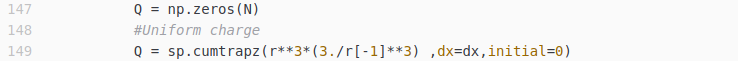
\includegraphics[width=\linewidth]{Q}
    \caption{Calculation of the charge as function of $r$ in the \textit{orbit.py} file. }
    \label{qcode}
\end{figure}
And that's all we need to do
knowing this we can proceed to use eq. \ref{vh} and calculate the Hartree potential. In fig. \ref{figvh} we show the function defined inside the orbit class to calculate the Hartree potential. Naturally it was also defined an attribute vh and vreal, vreal was made just to be able to compare with the analytic result considering uniform charge density.
\begin{figure}[h!]
    \centering
   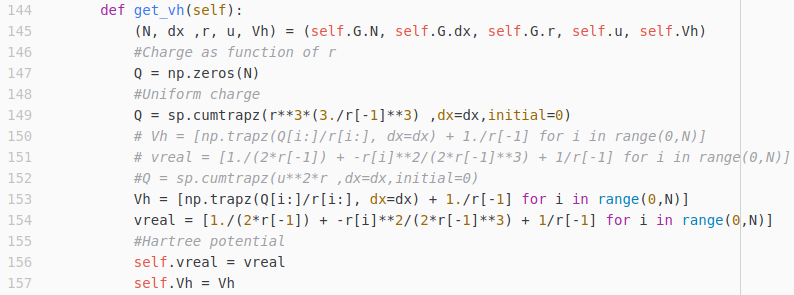
\includegraphics[width=\linewidth]{vh}
    \caption{Calculation of the Hartree potential as function of $r$ in the \textit{orbit.py} file. }
    \label{figvh}
\end{figure}
\section{Results}
If we consider the atoms to be uniformly charged spheres the solution we get is
\begin{figure}[h!]
    \centering
   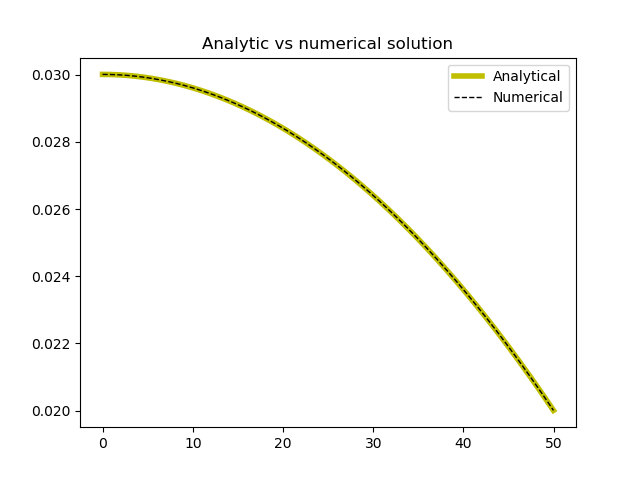
\includegraphics[width=0.7\linewidth]{comp}
    \caption{Numerical and analytical solutions considering the atom as a sphere of uniform charge. }
    \label{unif}
\end{figure}

If we use the $u(r)$ functions obtained with the program we get
\begin{figure}[h!]
    \centering
    \subfigure[$u_{1,l}$]{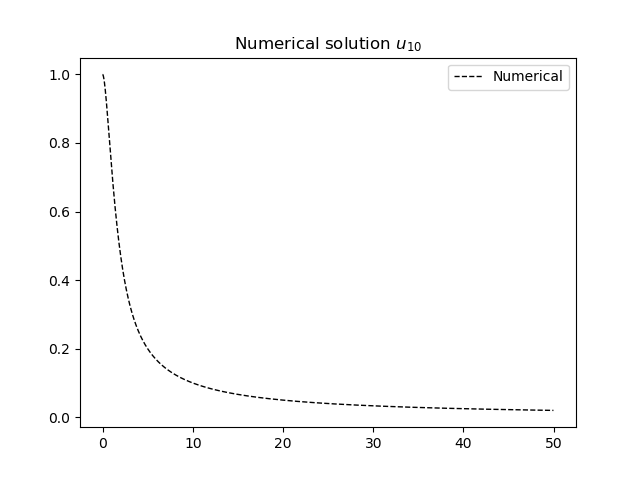
\includegraphics[height = 7cm]{num10}}
    \subfigure[$u_{2,l}$]{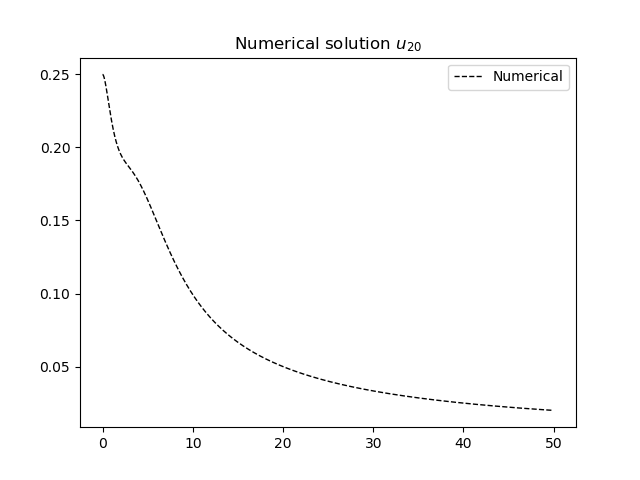
\includegraphics[height = 7cm]{num20}}
    \subfigure[$u_{3,l}$]{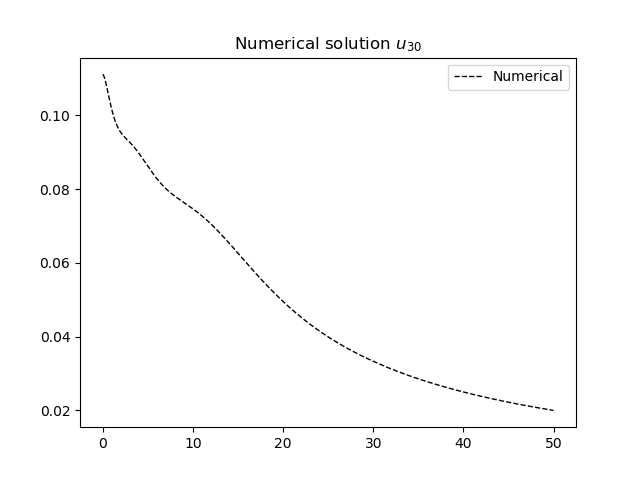
\includegraphics[height = 7cm]{num30}}
    \caption{Numerical solution for $V_H$ obtained using $u_{n0}$ for $n=1,2,3$. using eq.~\ref{vh} }
\label{results}
\end{figure}
\clearpage
%\begin{figure}[h!]
%    \centering
 %   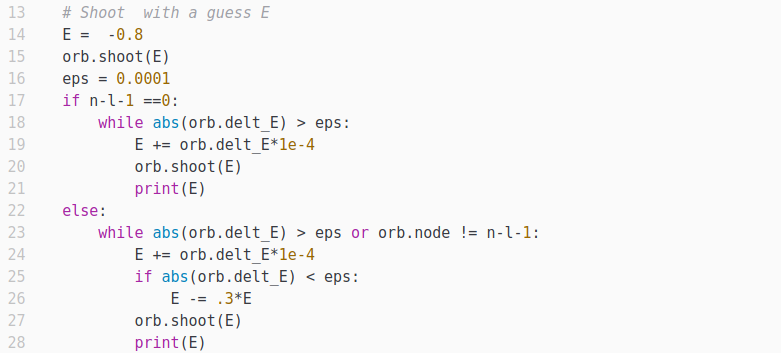
\includegraphics[width=\linewidth]{shoot}
%    \caption{Implementation of the algorithm to update the %energy until it converges to the desired value in %\textit{main.py}.}
%    \label{shoot}
%\end{figure}


%\begin{figure}
%    \centering
%    \subfigure[$u_{1,l}$]{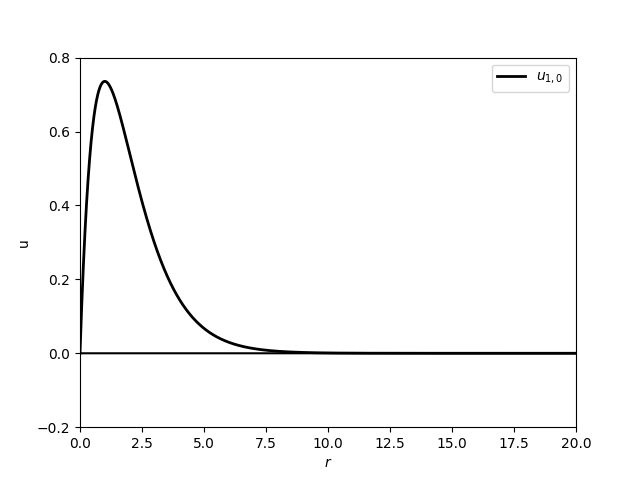
\includegraphics[height = %5.5cm]{u1.png}}
%    \caption{Plots of the hydrogen radial wavefunctions %for several values of $n$}\label{results}
%\end{figure}

\begin{thebibliography}{9}% 2nd arg is the width of the widest label.
\bibitem{zhangQ} Zhang, Q. (September 2014). Calculations of atomic multiplets across the periodic table (Master’s thesis). Retrieved from https://juser.fz-juelich.de/record/188242/files/FZJ-2015-01684.pdf.
\end{thebibliography}

\end{document}